\section[The ms+seqgen Approach]{The \code{ms+seqgen} Approach}
\label{sec:msseqgen}
\addcontentsline{toc}{section}{\thesection. The \code{ms+seqgen} Approach}

The \pkg{phyclust} incorporates two famous outsourced \proglang{C} programs
\pkg{ms} \citep{Hudson2002} and \pkg{seq-gen} \citep{Rambaut1997}.
The original source code and documents are available on the author's
websites.
For \pkg{ms},
the pdf file (download from the author's website) in the installed directory
\url{phyclust/doc/Documents/msdoc.pdf} or in the source code directory
\url{phyclust/inst/doc/Documents/msdoc.pdf}
For \pkg{seq-gen},
the html file (download from the author's website) in the installed directory
\url{phyclust/doc/Documents/Seq-Gen.v.1.3.2/Seq-Gen.Manual.html}
or in the source code directory
\url{phyclust/inst/doc/Documents/Seq-Gen.v.1.3.2/Seq-Gen.Manual.html}.

In the file \url{msdoc.pdf}, Dr. Hudson demonstrated examples to use \pkg{ms}
to generate coalescent trees and piped them to \pkg{seq-gen} to generate
sequences in the command mode.
The \pkg{phyclust} directly uses their options
in \proglang{R} functions \code{ms()} and \code{seqgen()}, and also modify
partial source code to use \proglang{R}'s library. Now, they can be
distributed with \proglang{R} across platforms without recompiling problems.
Moreover, combining with the \code{phyclust()} function, we can have a
\code{ms+seqgen+phyclust} approach in the
Section~\ref{sec:msseqgenphyclust} for simulation and bootstrap studies.




\subsection[Use the ms() function to generate trees]{Use the \code{ms()} function to generate trees}
\label{sec:ms}
\addcontentsline{toc}{subsection}{\thesubsection. Use the \code{ms()} function to generate trees}

Almost all options are carried from the command mode program \pkg{ms},
and input as an option \code{opts} in \code{ms()}.
Just call the function, it will return and show you all options.
\begin{Code}
> ms()
> ?ms
\end{Code}

The following is an example to generate a coalescent tree (\code{-T})
with 3 leaves (\code{nsam = 3})
and the population growth rate is 0.1
(\code{-G 0.1}). The \code{ms()} returns a text output
stored in an array by line, and the tree is in NEWICK format which can
be transfered by the \code{read.tree()} function in the \pkg{ape} package
\citep{Paradis2004}.
The \code{read.tree()} returns an object with class \code{phylo}
which can be drawn by the function \code{plot()} or \code{plot.phylo()}
in the \pkg{ape} package.
\begin{Code}
> set.seed(1234)
> (ret.ms <- ms(nsam = 3, opts = "-T -G 0.1"))
ms 3 1 -T -G 0.1 
//
(1: 0.568774938583,(2: 0.355949461460,3: 0.355949461460): 0.212825477123);
> (tree.anc <- read.tree(text = ret.ms[3]))

Phylogenetic tree with 3 tips and 2 internal nodes.

Tip labels:
[1] "1" "2" "3"

Rooted; includes branch lengths.
> tree.anc$tip.label <- paste("a", 1:3, sep = "")
> plot(tree.anc, type = "c")
> axisPhylo()
\end{Code}
\begin{figure}[h]
\begin{center}
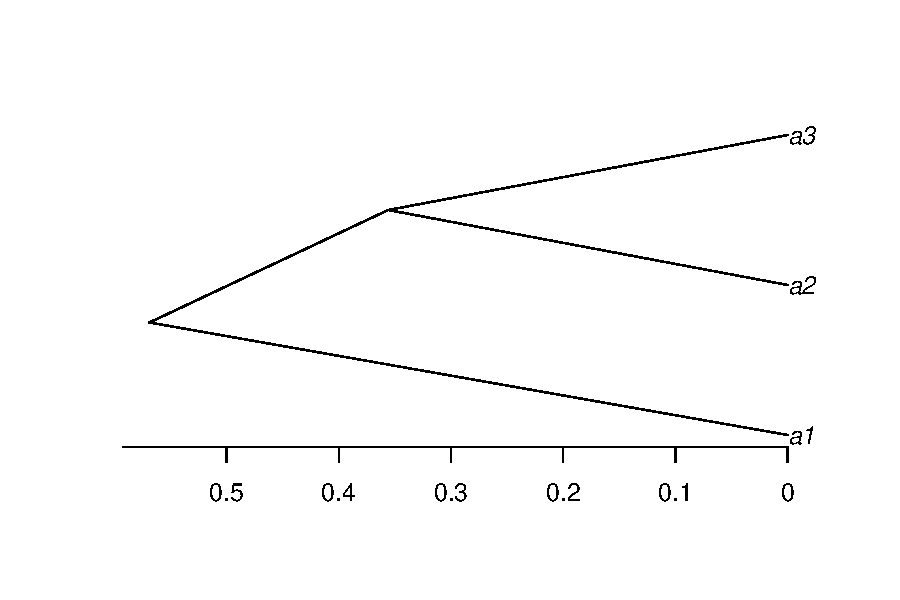
\includegraphics[width=5.0in]{./phyclust-graph/ms}
\caption{A diagram of a simple coalescent tree.}
\label{fig:ms}
\end{center}
\end{figure}




\subsection[Use the seqgen() function to generate sequences]{Use the \code{seqgen()} function to generate sequences}
\label{sec:seqgen}
\addcontentsline{toc}{subsection}{\thesubsection. Use the \code{seqgen()} function to generate sequences}

Almost all options are carried from the command mode program \pkg{seq-gen},
and input as an option \code{opts} in the \code{seqgen()} function.
Just call the function, it will return and show you all options.
The \code{seqgen()} function requires to take in a rooted tree either NEWICK
format or an object with class \code{phylo}.
\begin{Code}
> seqgen()
> ?seqgen
\end{Code}

In the following, I demonstrate the \code{ms+seqgen} approach
to generate sequences according a coalescent tree. This returns a character
vector with class {\color{red} \code{seqgen}} and contains 5 sequences, and
each has 40 bases (\code{-l40}). The option \code{-mHKY} is for the HKY85
model \citep{Hasegawa1985},
but it is equivalent to the JC69 model \citep{Jukes1969} if no further
setting is submitted.
\begin{Code}
> set.seed(123)
> ret.ms <- ms(nsam = 5, nreps = 1, opts = "-T")
> tree.anc <- read.tree(text = ret.ms[3])
> set.seed(123)
> seqgen(opts = "-mHKY -l40", newick.tree = ret.ms[3])
 5 40
1         CTCTCATTGGACGCACACTTTAGGGGGGGATTGCACTGCA
5         CTCTCTCTGGACGCACACTTTAAGGGGGGATTGAACTACA
2         CTCTTCGGGCTCGGATAAGTTTGGAGGGTTGTTCTCTACA
3         CTCTGAGTGCTCGGATTAGTTAGGGGGAATGACGTCTACA
4         CTCTTATCTCTCGGATAAGTTGGGGGTGATGGCTTTTACA
> set.seed(123)
> (ret.seq <- seqgen(opts = "-mHKY -l40", rooted.tree = tree.anc))
 5 40
1         CTCTCATTGGACGCACACTTTAGGGGGGGATTGCACTGCA
5         CTCTCTCTGGACGCACACTTTAAGGGGGGATTGAACTACA
2         CTCTTCGGGCTCGGATAAGTTTGGAGGGTTGTTCTCTACA
3         CTCTGAGTGCTCGGATTAGTTAGGGGGAATGACGTCTACA
4         CTCTTATCTCTCGGATAAGTTGGGGGTGATGGCTTTTACA
> str(ret.seq)
Class 'seqgen'  chr [1:6] " 5 40" "1         CTCTCATTGGACGCACACTTTAGGGGGG ...
\end{Code}

The \code{seqgen()} function does not necessary to take in a tree from
the \code{ms()} function,
but the \code{ms()} function provides varied ways to construct a tree in
different shapes based on the coalescent theory.
The \code{seqgen()} function also allows to input an ancestral sequence and
evolves the sequence along the given tree by inputing an option \code{input}.
Originally, it uses a file to store the information in the \pkg{seq-gen}
package, and I implement a function to utilize this option described in the
Section~\ref{sec:ancestral}.




\subsection[Give an ancestral sequence to the ms+seqgen]{Give an ancestral sequence to the \code{ms+seqgen}}
\label{sec:ancestral}
\addcontentsline{toc}{subsection}{\thesubsection. Give an ancestral sequence to the \code{ms+seqgen} \vspace{-0.3cm}}

The \pkg{phyclust} package provides two functions \code{gen.seq.HKY()} and
\code{gen.seq.SNP()} to implement the \code{ms+seqgen}
approach under a wide-range parameters. A rooted tree is required and an
ancestral sequence is an option.

The following example generates a tree first, and gives an ancestral
sequence \code{anc.HKY}. The process in the \code{seqgen()} will follow
the parameters $\kappa$ (\code{kappa}) and
$\pi_{A}, \pi_{G}, \pi_{C}, \pi_{T}$ (\code{pi.HKY})
to evolve the ancestral sequence (\code{anc.HKY}).
\begin{Code}
> # Generate a tree
> set.seed(1234)
> ret.ms <- ms(nsam = 5, nreps = 1, opts = "-T")
> tree.ms <- read.tree(text = ret.ms[3])
> 
> # Generate nucleotide sequences
> (anc.HKY <- rep(0:3, 3))
 [1] 0 1 2 3 0 1 2 3 0 1 2 3
> paste(nid2code(anc.HKY, lower.case = FALSE), collapse = "")
[1] "AGCTAGCTAGCT"
> pi.HKY <- c(0.2, 0.2, 0.3, 0.3)
> kappa <- 1.1
> L <- length(anc.HKY)
> set.seed(1234)
> (HKY.1 <- gen.seq.HKY(tree.ms, pi.HKY, kappa, L, anc.seq = anc.HKY))
 5 12
1         AGCTTGACCGGC
3         AGCTTCACCGGT
2         ACCTCGCTAGCT
4         ACGACGCTCGCT
5         CCTACGCTAGCT
\end{Code}

Note that the details of the \code{gen.seq.HKY()} may be a good example
for advance users to develop more flexible conditions such as recombinations,
migrations and island models. Basically, it passes an option \code{input} to
the \code{seqgen()}, and it can be the ancestral sequence or other
options used in the \pkg{seq-gen} program.
The \code{input} takes in a character vector (including the tree)
where each element contains one line, and it will be store/write to
a temporary file in the \code{seqgen()} for further processing.
\begin{Code}
### Source code from gen.seq.HKY().
        L <- length(anc.seq)
        mu <- paste(nid2code(anc.seq, lower.case = FALSE), collapse = "")
        seqname <- paste("Ancestor  ", collapse = "")
        input <- c(paste(" 1", length(anc.seq), sep = " "), paste(seqname, 
            mu, sep = ""), 1, write.tree(rooted.tree, digits = 12))
        opts <- paste("-mHKY", " -t", ts.tv, " -f", paste(pi[c(1, 
            3, 2, 4)], collapse = ","), " -l", L, " -s", rate.scale, 
            " -u", ttips + 1, " -k1", " -q", sep = "")
        ret <- seqgen(opts, input = input)

### Source code from seqgen().
        if (!is.null(newick.tree)) {
            write(newick.tree, file = temp.file.ms, sep = "")
        }
        else if (!is.null(input)) {
            write(input, file = temp.file.ms, sep = "\n")
        }
        else {
            stop("A newick or rooted/phylo tree is required.")
        }
\end{Code}

